\documentclass[11pt,a4paper]{article}

% ── Packages ──────────────────────────────────────────────────────────────────
\usepackage[T1]{fontenc}
\usepackage[utf8]{inputenc}
\usepackage{helvet}
\renewcommand{\familydefault}{\sfdefault}   % Arial-like sans-serif font
\usepackage[margin=2.5cm]{geometry}
\usepackage{hyperref}
\usepackage{listingsutf8}
\usepackage{xcolor}
\usepackage{enumitem}
\usepackage{titlesec}
\usepackage{parskip}
\usepackage{booktabs}
\usepackage{graphicx}
\usepackage{amsmath}
\usepackage{fancyhdr}
\usepackage[title]{appendix}

% ── Colors ────────────────────────────────────────────────────────────────────
\definecolor{codebg}{HTML}{F5F5F5}
\definecolor{codeframe}{HTML}{CCCCCC}
\definecolor{keyword}{HTML}{0000CC}
\definecolor{comment}{HTML}{007700}
\definecolor{string}{HTML}{CC0000}
\definecolor{uu-red}{HTML}{990000}

% ── Listings style ────────────────────────────────────────────────────────────
\lstdefinestyle{docker}{
  language=bash,
  basicstyle=\ttfamily\small,
  backgroundcolor=\color{codebg},
  frame=single,
  rulecolor=\color{codeframe},
  breaklines=true,
  breakatwhitespace=true,
  columns=fullflexible,
  keepspaces=true,
  showstringspaces=false,
  commentstyle=\color{comment},
  keywordstyle=\color{keyword}\bfseries,
  stringstyle=\color{string},
  numbers=left,
  numberstyle=\tiny\color{gray},
  numbersep=8pt,
  tabsize=2,
}

\lstdefinestyle{yaml}{
  language=bash,
  basicstyle=\ttfamily\small,
  backgroundcolor=\color{codebg},
  frame=single,
  rulecolor=\color{codeframe},
  breaklines=true,
  columns=fullflexible,
  keepspaces=true,
  showstringspaces=false,
  morecomment=[l]{\#},
  commentstyle=\color{comment},
  numbers=left,
  numberstyle=\tiny\color{gray},
  numbersep=8pt,
  tabsize=2,
}

\lstdefinestyle{shell}{
  language=bash,
  basicstyle=\ttfamily\small,
  backgroundcolor=\color{codebg},
  frame=single,
  rulecolor=\color{codeframe},
  breaklines=true,
  columns=fullflexible,
  keepspaces=true,
  showstringspaces=false,
}

\lstdefinestyle{python}{
  language=Python,
  basicstyle=\ttfamily\small,
  backgroundcolor=\color{codebg},
  frame=single,
  rulecolor=\color{codeframe},
  breaklines=true,
  breakatwhitespace=true,
  columns=fullflexible,
  keepspaces=true,
  showstringspaces=false,
  commentstyle=\color{comment},
  keywordstyle=\color{keyword}\bfseries,
  stringstyle=\color{string},
  numbers=left,
  numberstyle=\tiny\color{gray},
  numbersep=8pt,
  tabsize=4,
}

% ── Section title formatting ──────────────────────────────────────────────────
\lstset{inputencoding=utf8, extendedchars=true}
\titleformat{\section}{\large\bfseries\color{black}}{\thesection}{1em}{}
\titleformat{\subsection}{\normalsize\bfseries}{\thesubsection}{1em}{}

% ── Header / Footer ───────────────────────────────────────────────────────────
\pagestyle{fancy}
\fancyhf{}
\lhead{\small Data Engineering II -- Assignment 2}
\rhead{\small Uppsala University}
\cfoot{\thepage}

% ── Hyperref setup ────────────────────────────────────────────────────────────
\hypersetup{
  colorlinks=true,
  linkcolor=black,
  urlcolor=blue,
}

% ─────────────────────────────────────────────────────────────────────────────
\begin{document}

% ── Title page ────────────────────────────────────────────────────────────────
\begin{titlepage}
  \centering
  \vspace*{2cm}
  {\large Uppsala University\\[0.3em]
   Department of Information Technology\\[2cm]}
  {\LARGE\bfseries Assignment 2\\[0.5em]}
  {\Large Data Stream Processing\\[2cm]}
  {\large Course: Data Engineering II\\[1.5cm]}
  {\normalsize Arnab Kumar Ghosh\\[0.5cm]}
  {\normalsize \today\\[3cm]}
  \vfill
\end{titlepage}

\tableofcontents
\newpage

% =============================================================================
\section{Task 1: Setting up Apache Pulsar}
% =============================================================================

Apache Pulsar is an open-source distributed messaging and streaming platform.
Before I could produce or consume messages, I needed a running Pulsar service.
There are two ways to do this: installing Pulsar directly on the VM, or running it
inside a Docker container. In this task, I used the Docker method because it is
faster to set up and keeps the VM clean.

\subsection{Setting up the VM}

Before starting Pulsar, the VM needs Java and Docker. I wrote a setup script
\texttt{setup\_vm.sh} to install all prerequisites automatically.

The script does the following steps:

\begin{itemize}[leftmargin=1.5cm]
  \item Updates all system packages with \texttt{apt update} and \texttt{apt upgrade}.
  \item Installs the Java Runtime Environment, which Pulsar requires to run.
  \item Installs Docker CE using Docker's official repository and starts the Docker service.
  \item Installs \texttt{python3-pip} and the
        \texttt{pulsar-client==2.9.4} Python library.
\end{itemize}

\subsection{Setting up Pulsar in a container in a VM}

Once the VM was ready, I started Apache Pulsar in standalone mode using the
official Docker image. Standalone mode runs the broker, BookKeeper, and
ZooKeeper all in one process, which is enough for development and testing.

\begin{lstlisting}[style=shell, caption={Starting Apache Pulsar in a Docker container}]
docker run -it \
  -p 6650:6650 \
  -p 8080:8080 \
  --mount source=pulsardata,target=/pulsar/data \
  --mount source=pulsarconf,target=/pulsar/conf \
  apachepulsar/pulsar:2.9.4 bin/pulsar standalone
\end{lstlisting}

\begin{itemize}[leftmargin=1.5cm]
  \item \texttt{-p 6650:6650} -- Exposes the Pulsar broker port so clients
        can connect to it.
  \item \texttt{-p 8080:8080} -- Exposes the Pulsar admin REST API port.
  \item \texttt{--mount source=pulsardata} -- Mounts a named Docker volume
        for persistent message data. Data survives even if the container is restarted.
  \item \texttt{--mount source=pulsarconf} -- Mounts a separate volume for
        Pulsar configuration files.
  \item \texttt{bin/pulsar standalone} -- Starts Pulsar in standalone mode.
\end{itemize}

\subsection{Running the Program}

When Pulsar starts successfully, the logs show a JSON status block with
\texttt{"alive": true} and regular HTTP request lines from the admin API.
This confirms that the broker is running and healthy.

\begin{figure}[h!]
  \centering
  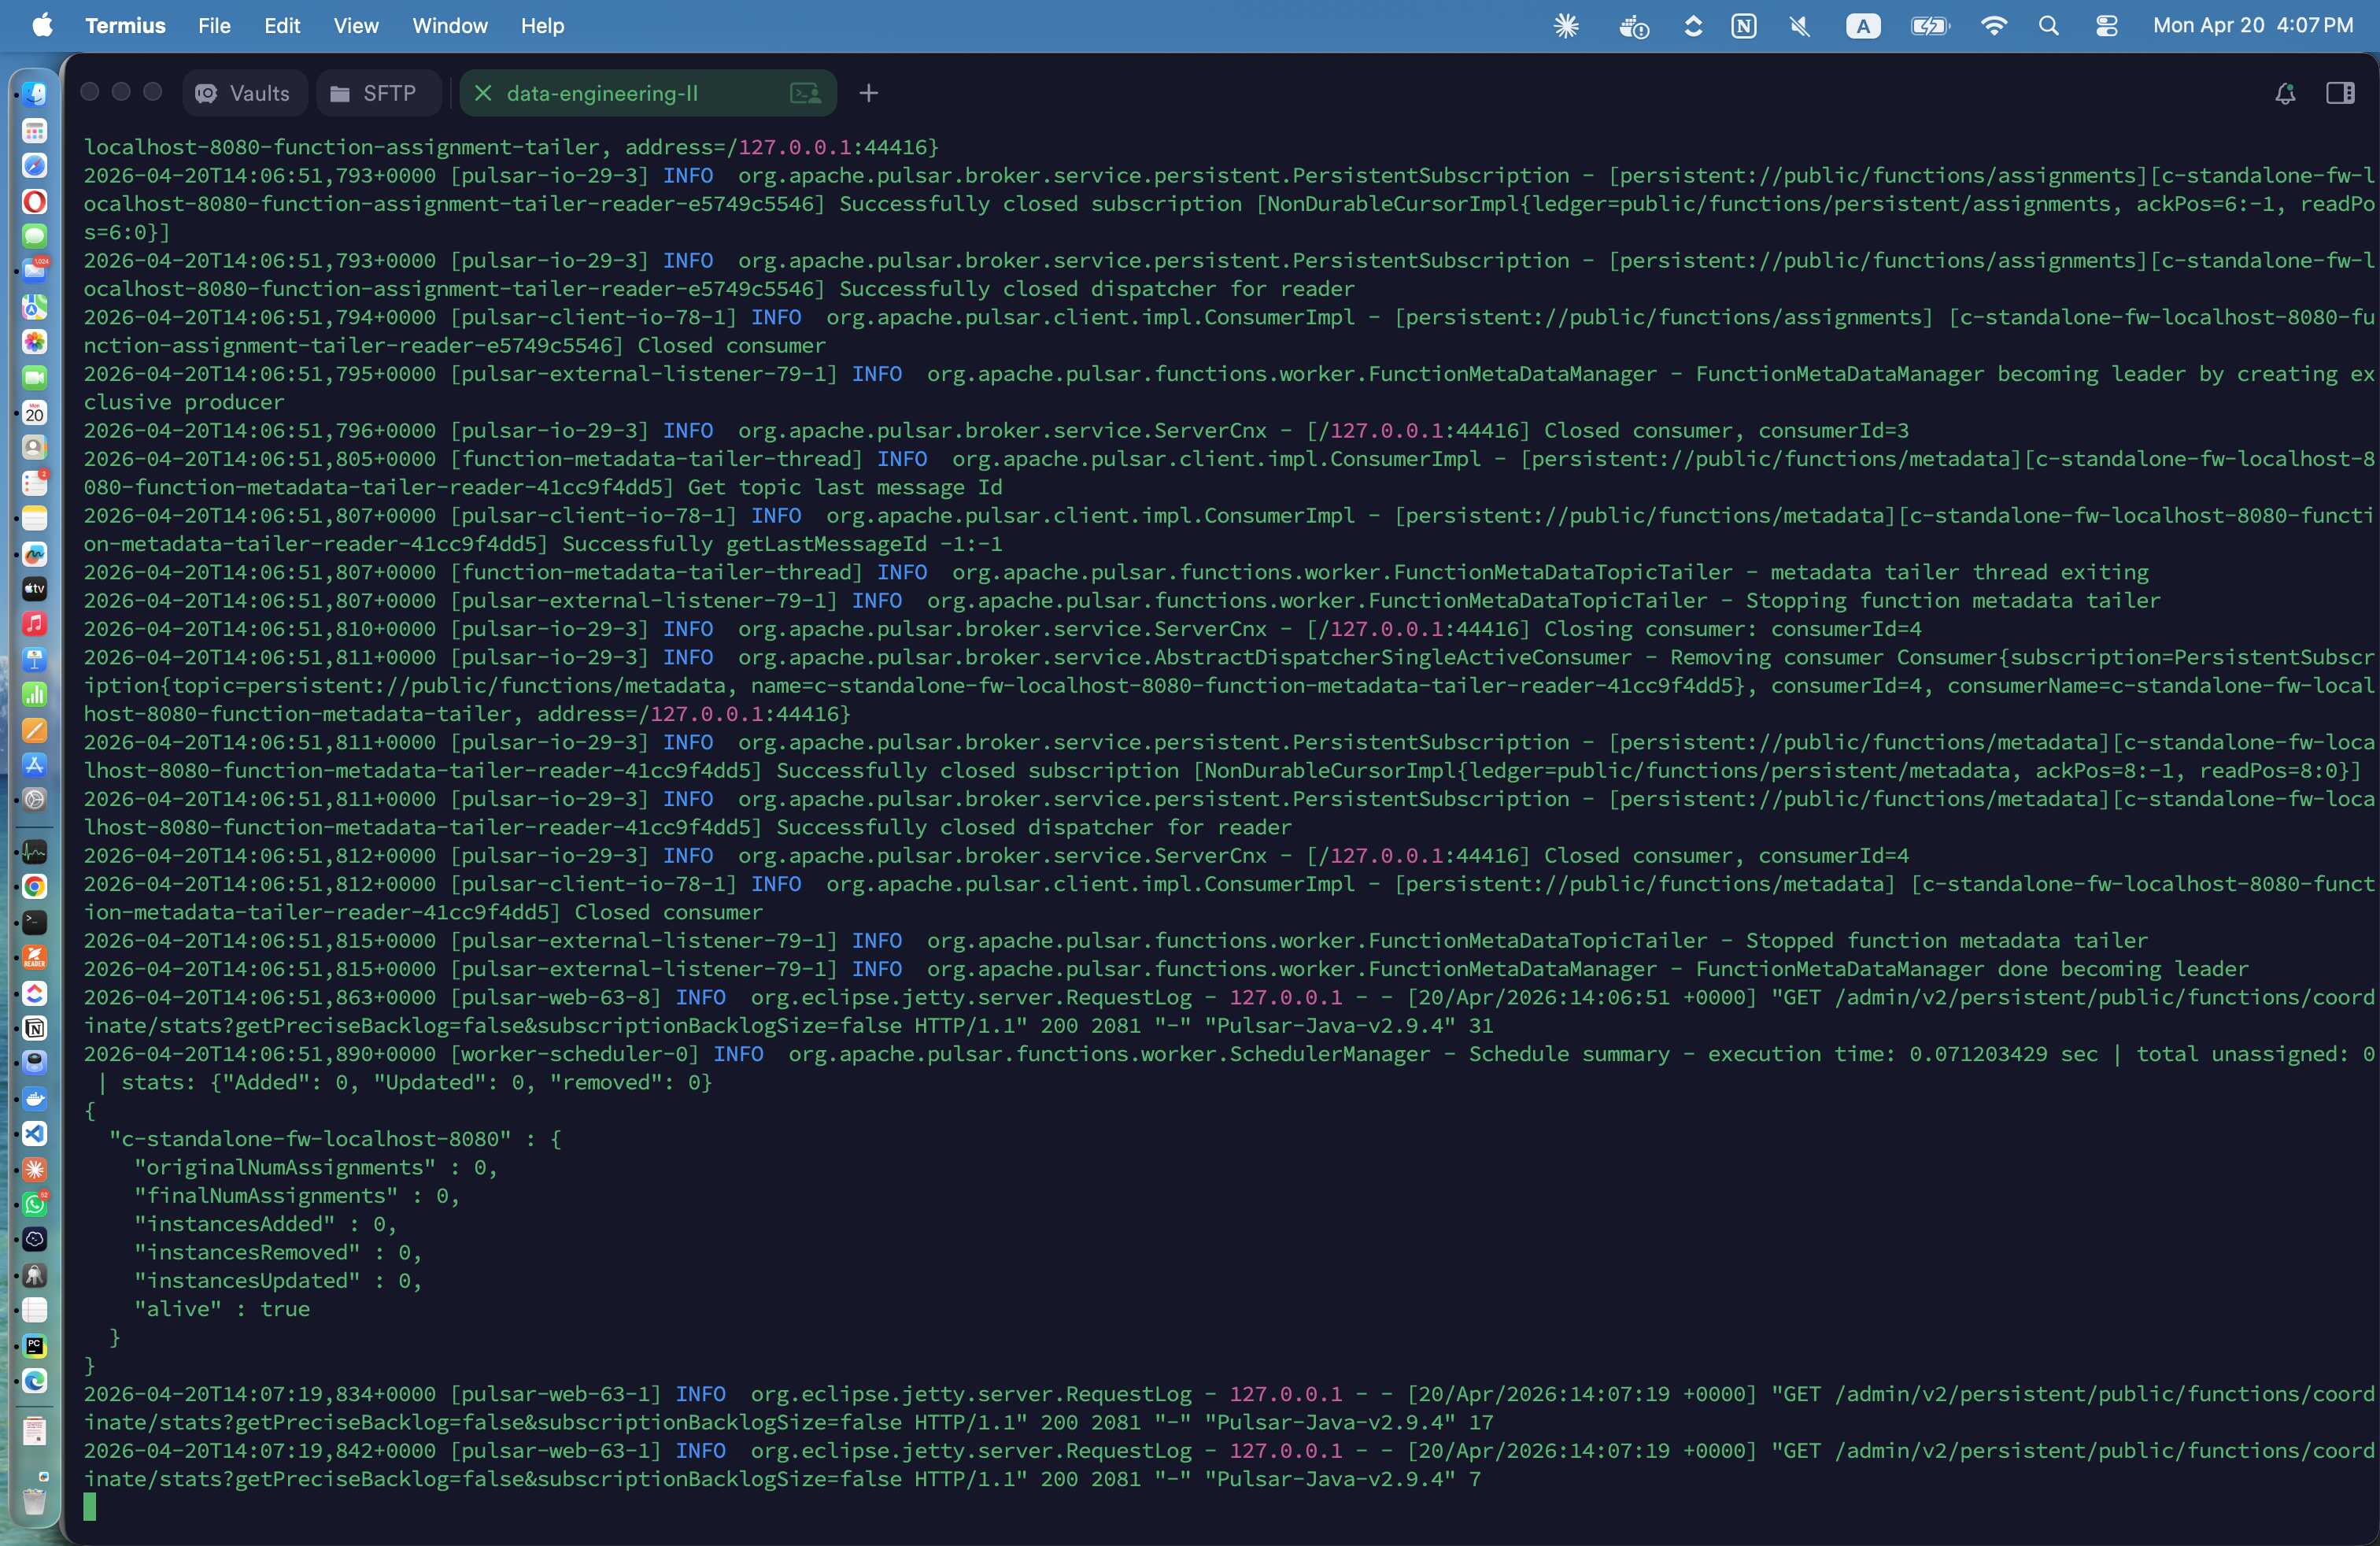
\includegraphics[width=\textwidth]{task-1-pulsar-setup.png}
  \caption{Apache Pulsar running successfully in standalone mode inside a Docker container.}
  \label{fig:task1-pulsar}
\end{figure}

\newpage

% =============================================================================
\section{Task 2: Producing and Consuming Messages}
% =============================================================================

% ──────────────────────────────────────────────────────────────────────────────
\subsection{A: Running Apache Pulsar, consumer and producer on a single
machine}

With Pulsar running, I wrote a producer and a consumer. In this part,
both programs run on the same VM that hosts the Pulsar broker.

\subsubsection{Installing the Python Client Library}

Before running any Python code, the Pulsar client library must be installed.
The setup script already handles this, but the command is:

\begin{lstlisting}[style=shell]
pip install pulsar-client==2.9.4
\end{lstlisting}

\subsubsection{The Consumer}

The consumer subscribes to a topic and waits for messages. It acknowledges
each message it receives so Pulsar knows the message was processed.
The implementation of \texttt{consumer-task-2-A.py} is shown in Appendix \ref{app:code}.

\subsubsection{The Producer}

The producer connects to the same topic and sends one message.
The implementation of \texttt{producer-task-2.py} is shown in Appendix \ref{app:code}.

\subsubsection{Running the Programs}

I opened three separate SSH sessions to the VM. Pulsar was already running
in the first session. I started the consumer in the second session and left it
waiting. I then ran the producer in the third session.

\begin{lstlisting}[style=shell, caption={Running the consumer and producer}]
# Terminal 2: start the consumer and keep it waiting
python3 consumer-task-2-A.py

# Terminal 3: run the producer to send a message
python3 producer-task-2.py
\end{lstlisting}

As soon as the producer sent the message, the consumer printed:

\begin{lstlisting}[style=shell]
Received message : 'b'Welcome to Data Engineering Course!''
\end{lstlisting}

This confirms that the message was successfully delivered through the Pulsar broker.

\begin{figure}[h!]
  \centering
  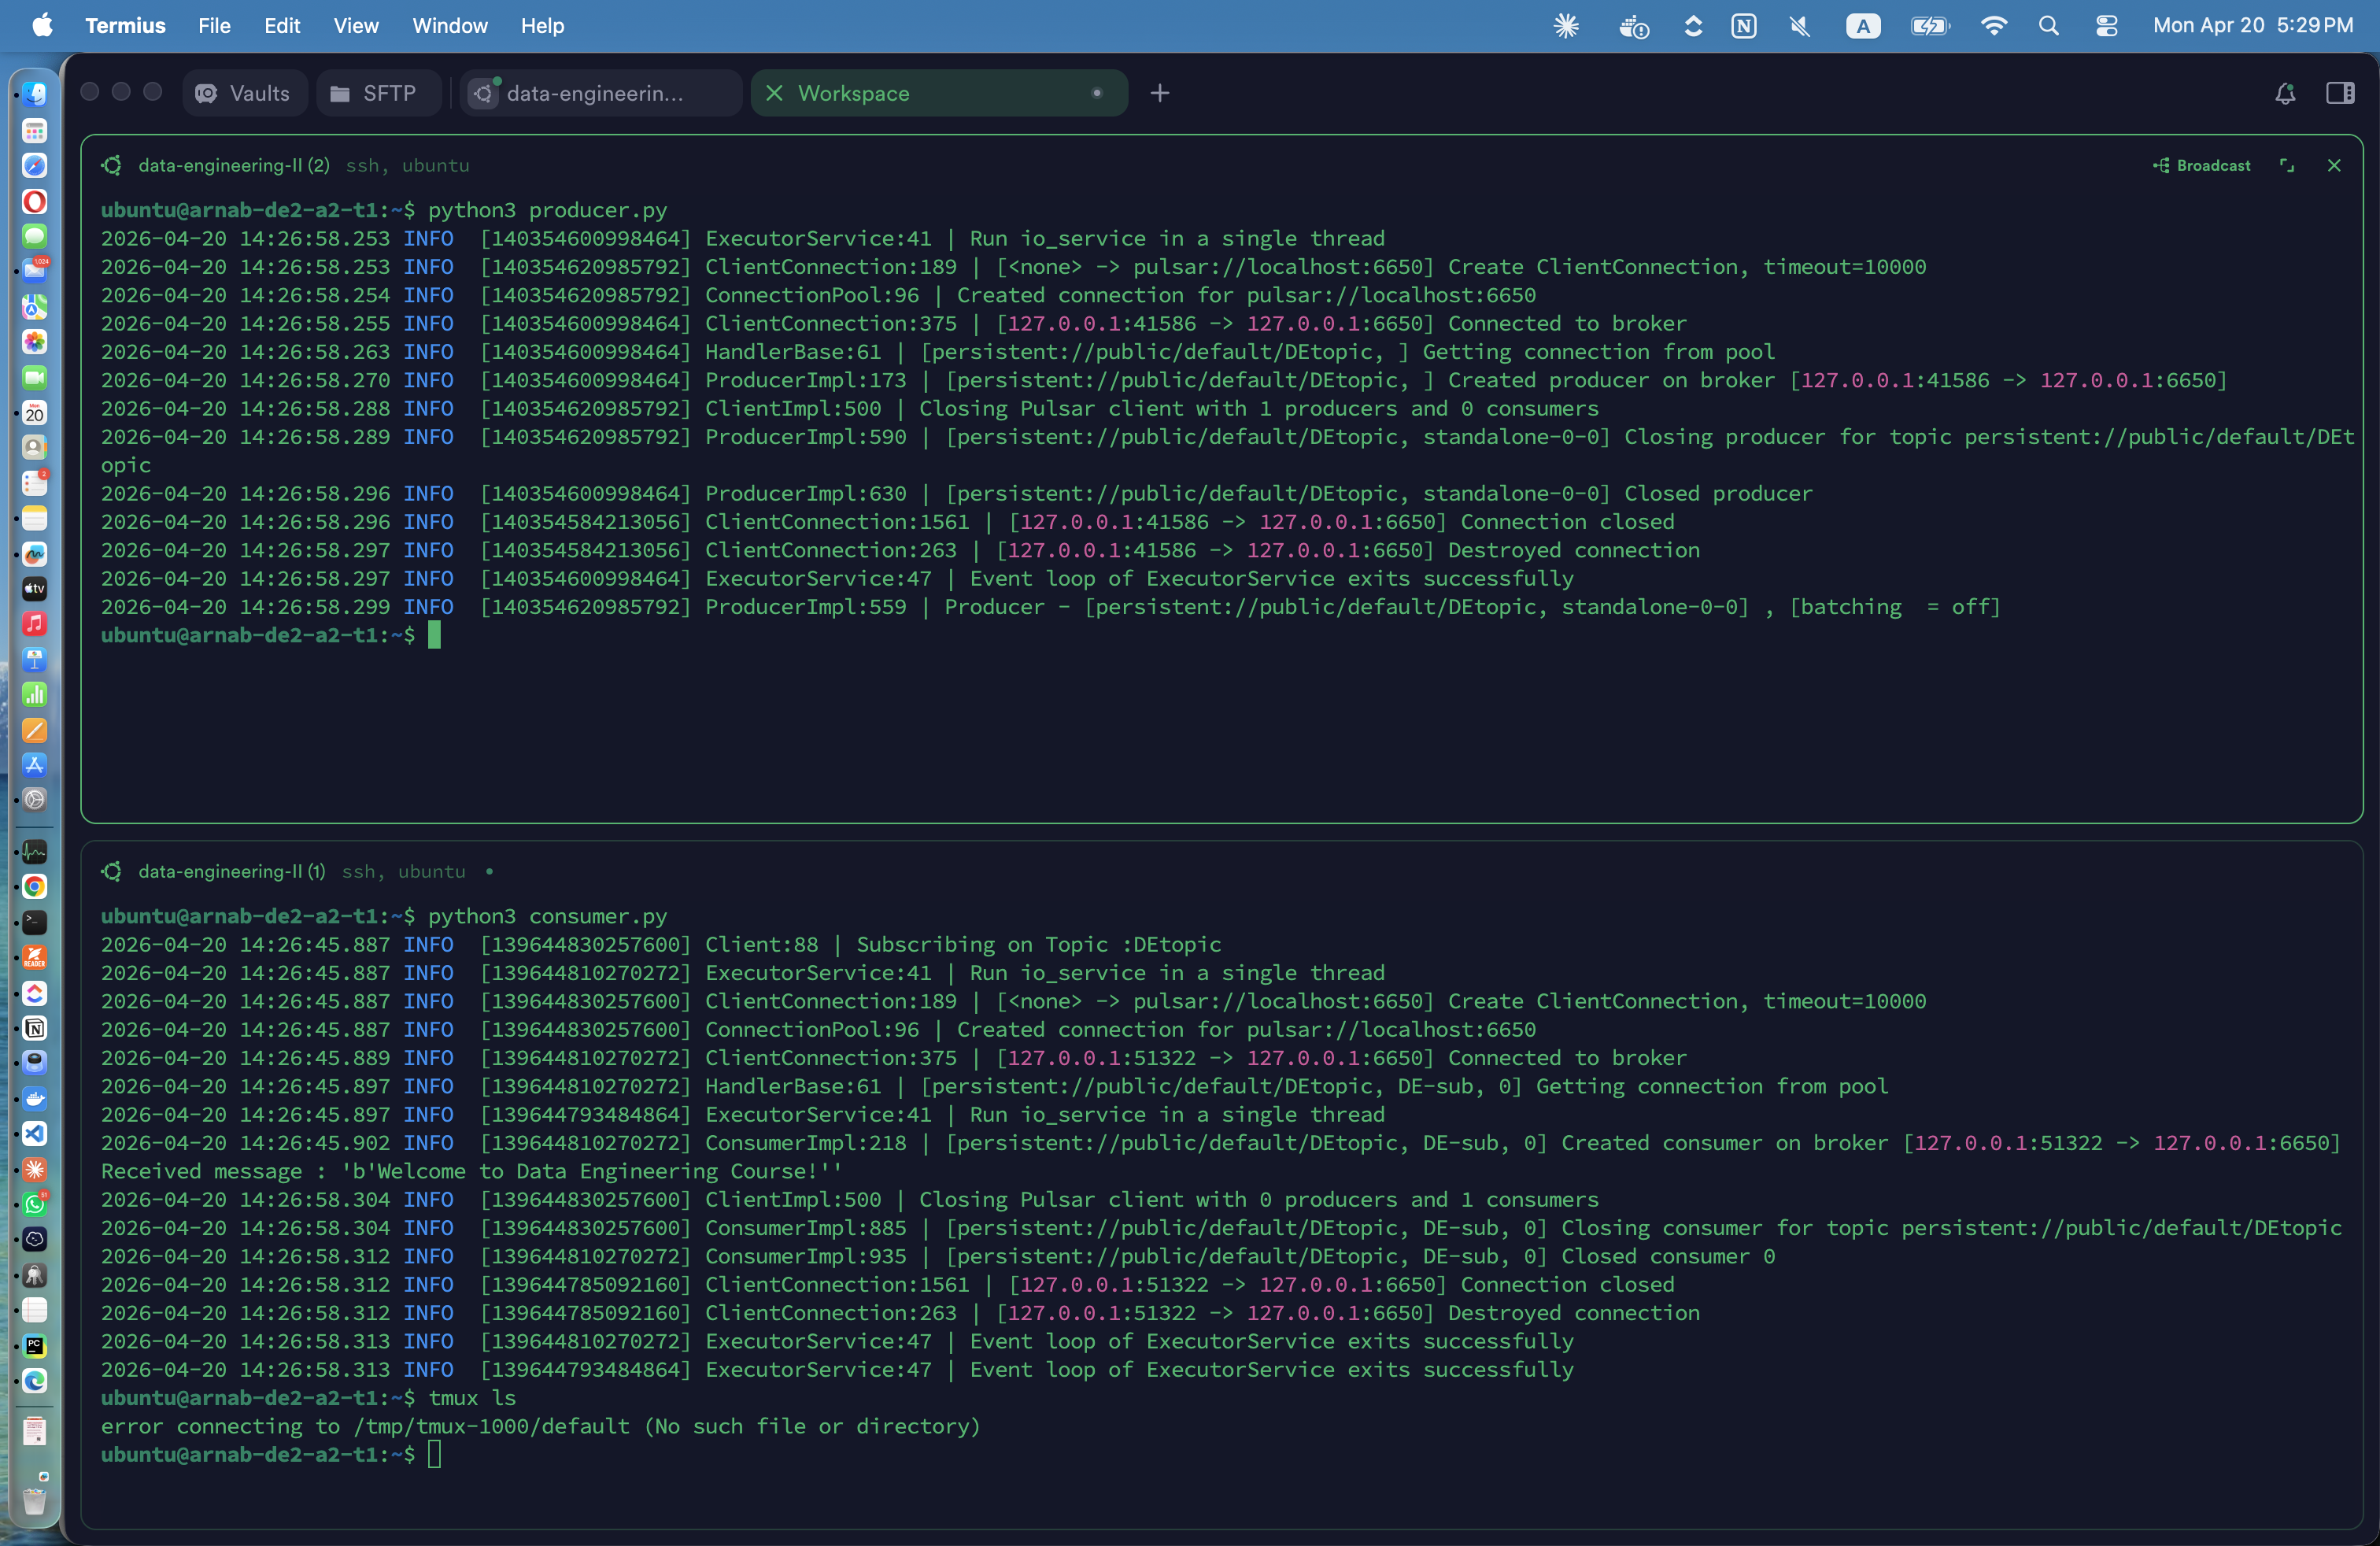
\includegraphics[width=\textwidth]{task-2-consumer-producer-message.png}
  \caption{Consumer receiving a message sent by the producer on the same machine.}
  \label{fig:task2a}
\end{figure}

\newpage

% ──────────────────────────────────────────────────────────────────────────────
\subsection{B: Running Apache Pulsar, consumer and producer on multiple
machines}

In this part, the setup is distributed across two separate virtual machines on the Swedish Science Cloud (NAISS).
Apache Pulsar and the producer run on \textbf{VM A}, while the consumer runs on \textbf{VM B}.

\subsubsection{Infrastructure}

\begin{itemize}[leftmargin=1.5cm]
  \item \textbf{VM A} (\texttt{arnab-de2-a2-t1}): private IP \texttt{192.168.2.198}: runs
        the Pulsar broker in Docker and the producer.
  \item \textbf{VM B} (\texttt{arnab-de2-a2-t2}): private IP \texttt{192.168.2.166}: runs
        the consumer only. No Docker is required on this machine.
\end{itemize}

\subsubsection{Which IP Address to Use?}

The private IP address should be used. Both VMs are on the same Swedish Science Cloud
(NAISS) internal network, so VM B can reach VM A directly using the private IP
(\texttt{192.168.2.198}). The traffic stays inside the data centre and does not leave
the internal network. The public floating IP (\texttt{130.*.*.*}) routes traffic externally
and would require opening port 6650 in the security group, which adds unnecessary
exposure. Therefore, I used the private IP address in the consumer's broker URL.

\subsubsection{Starting Pulsar on VM A}

I used the same Docker command as in Task 1 without any changes:

\begin{lstlisting}[style=shell, caption={Starting Pulsar on VM A -- same command as Task 1}]
docker run -it \
  -p 6650:6650 \
  -p 8080:8080 \
  --mount source=pulsardata,target=/pulsar/data \
  --mount source=pulsarconf,target=/pulsar/conf \
  apachepulsar/pulsar:2.9.4 bin/pulsar standalone
\end{lstlisting}

Since both VMs are on the same Swedish Science Cloud (NAISS) private network, VM B can connect to the broker
on VM A's private IP even with the default port binding.

\subsubsection{The Consumer on VM B}
On VM B, only the \texttt{pulsar-client} library is needed:

\begin{lstlisting}[style=shell]
pip3 install pulsar-client==2.9.4
\end{lstlisting}

The consumer script is identical in logic to Part A, but the broker URL points to
VM A's private IP instead of \texttt{localhost}.
The implementation of \texttt{consumer-task-2-B.py} is shown in Appendix \ref{app:code}.


\subsubsection{Running the Programs}

I started the consumer on VM B first, then ran the producer on VM A.
The consumer immediately printed the received message, confirming that
the message flowed correctly across the two machines through the Pulsar broker.

\begin{figure}[h!]
  \centering
  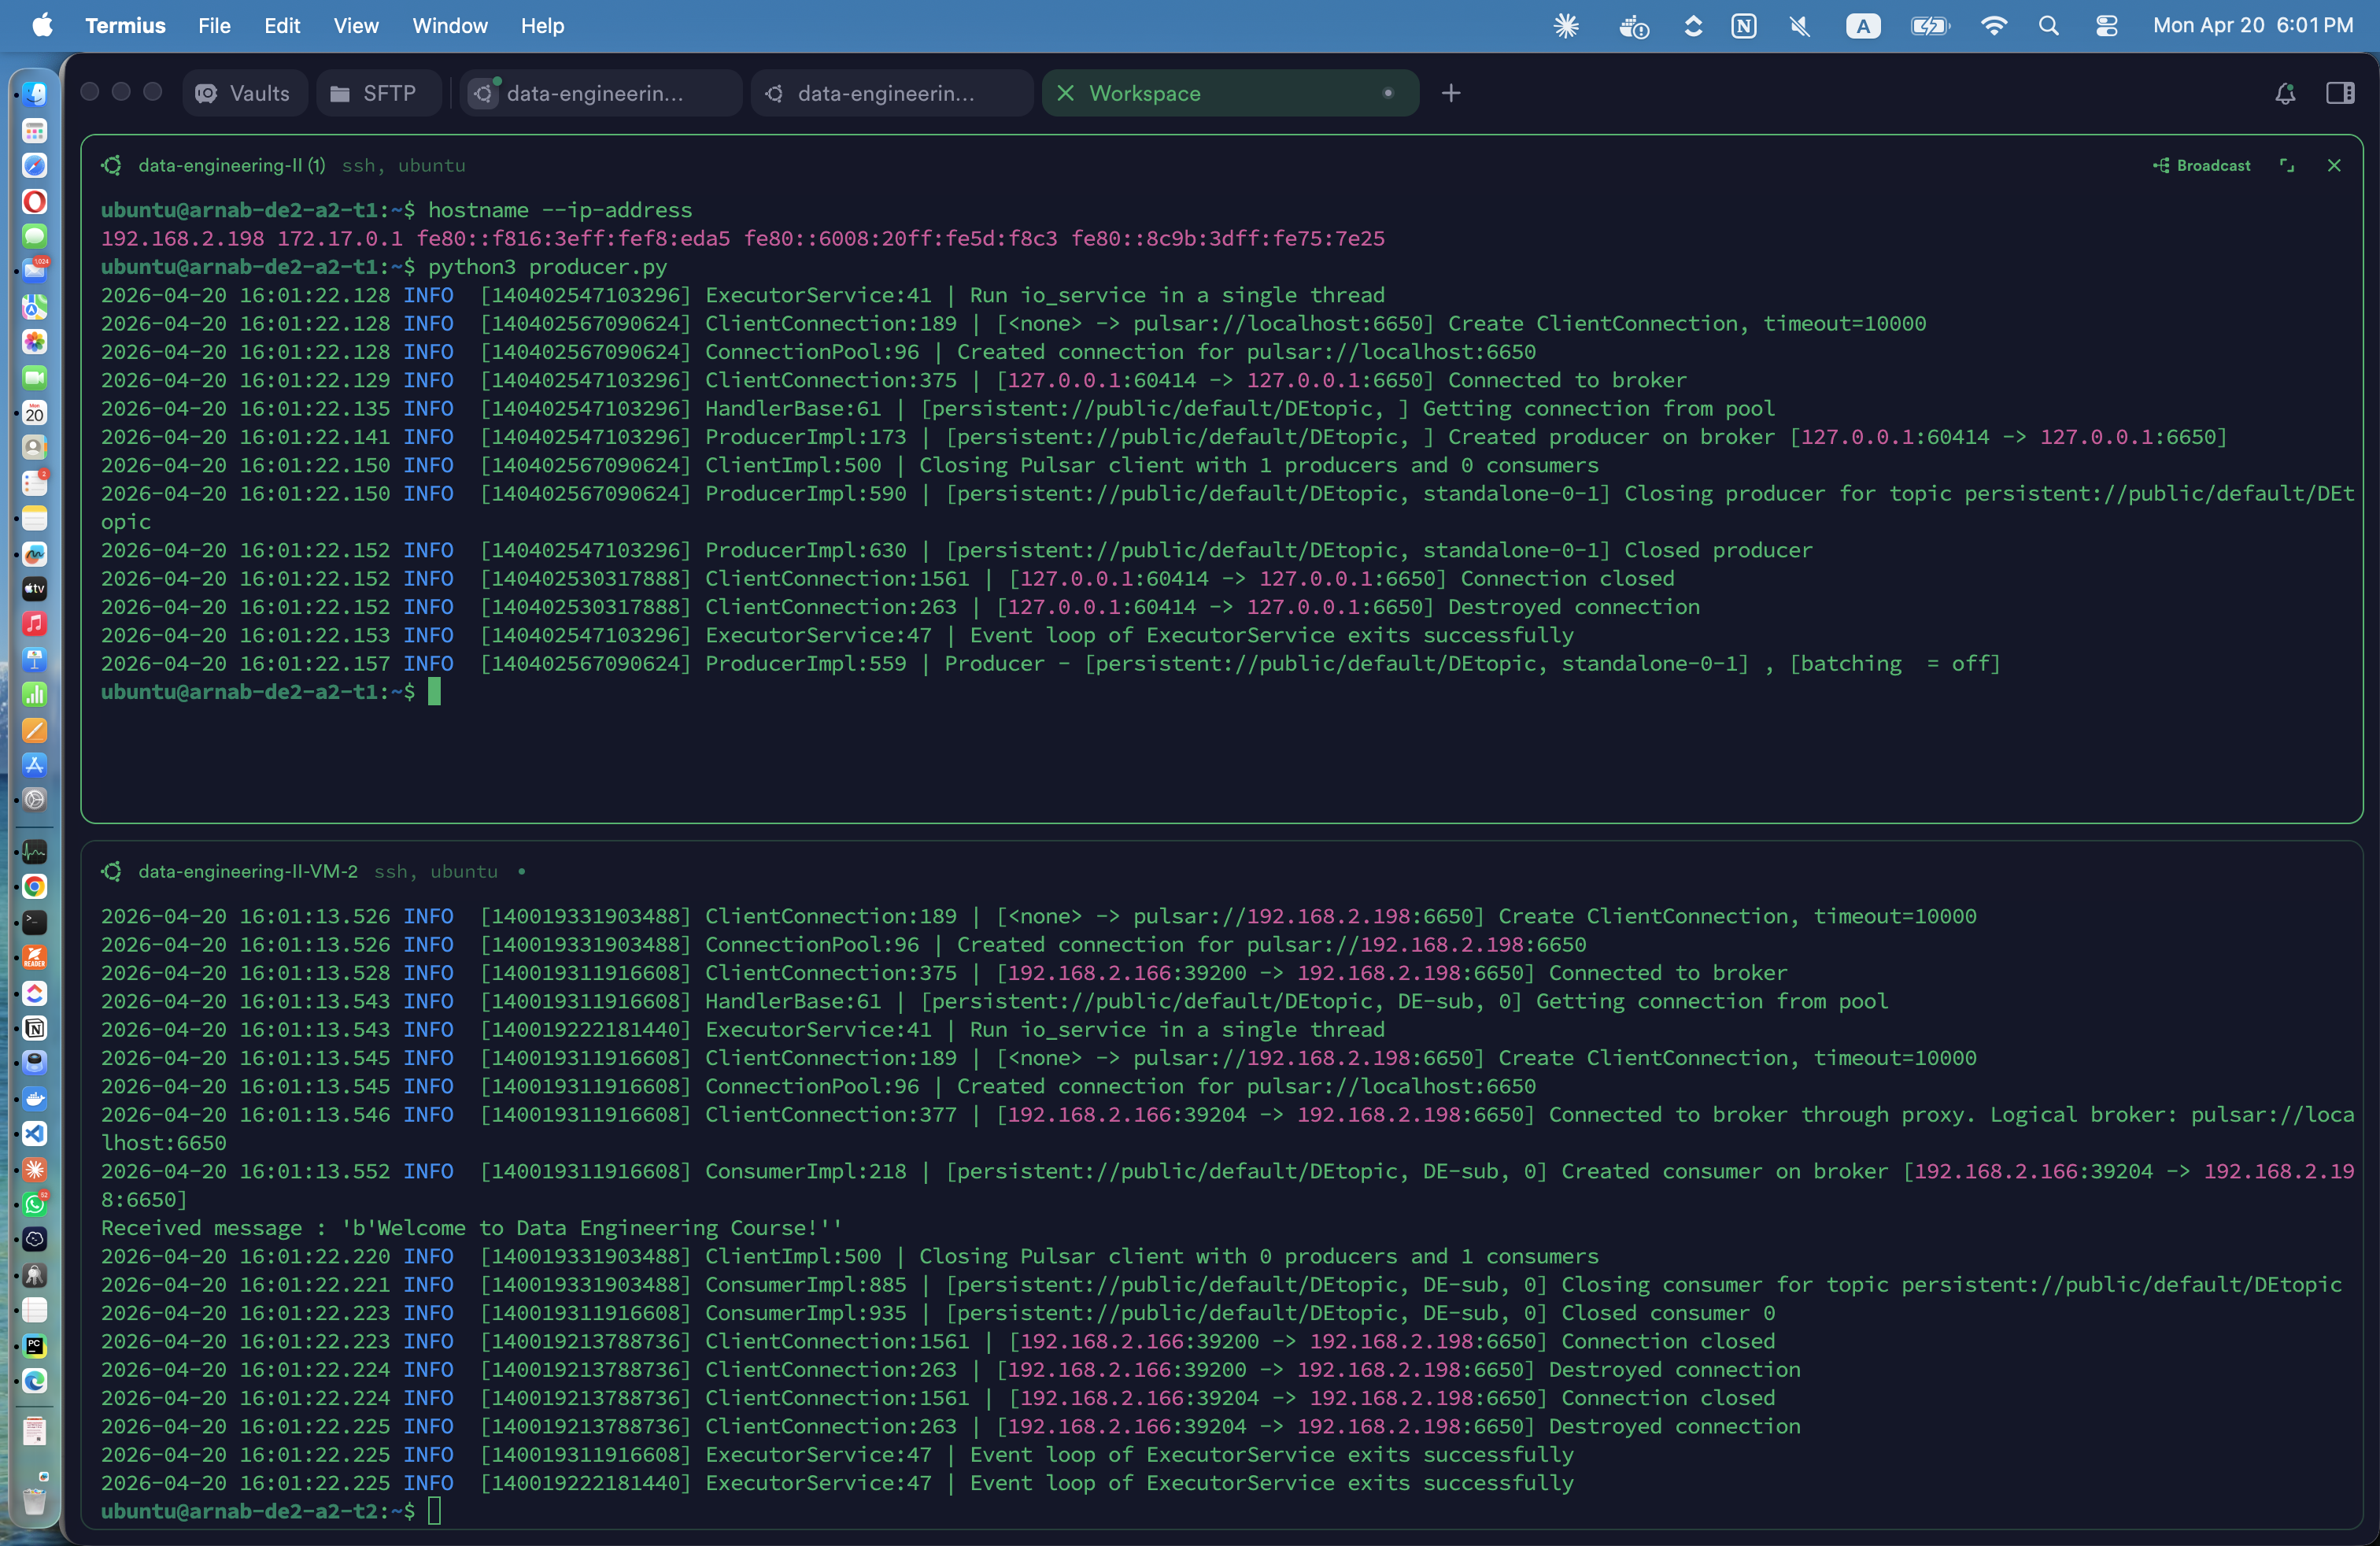
\includegraphics[width=\textwidth]{task-2-B-consumer-producer-message.png}
  \caption{Consumer on VM B (\texttt{arnab-de2-a2-t2}) receiving a message produced on VM A (\texttt{arnab-de2-a2-t1}), demonstrating cross-machine message delivery via Apache Pulsar.}
  \label{fig:task2b}
\end{figure}

\newpage

% =============================================================================
\section{Task 3: Conceptual Questions}
% =============================================================================

\subsection*{1. What are the primary trade-offs when deploying Apache Pulsar in a Docker container versus a native environment?}

In Task 1, I chose Docker because it let me start Pulsar with one command and did not
change anything on the VM. The same \texttt{docker run} command works on any machine,
so the setup is easy to repeat. The main problem I noticed is that Docker uses its own
internal network. By default, Pulsar tells clients to connect to its internal IP, which
other machines cannot reach. Setting \texttt{PULSAR\_ADVERTISED\_ADDRESS} fixes this.

Running Pulsar directly on the VM is faster and has simpler networking. The downside is
that Java, ZooKeeper, BookKeeper, and Pulsar all need to be installed manually. This takes
more time and is harder to repeat on a second machine.

\subsection*{2. What features does Apache Pulsar support that previous distributed streaming frameworks, such as Kafka, do not?}

Apache Pulsar has several features that Kafka does not have natively:

 \textbf{Unified messaging}: Pulsar supports both message queuing and publish-subscribe in
        one system. Kafka is mainly a publish-subscribe log.

  \textbf{Multi-tenancy}: Pulsar has built-in support for multiple tenants with
        separate access control and resource limits. Kafka has no such feature.
 
  \textbf{Pulsar Functions}: a simple built-in way to run stream processing logic
        without needing a separate engine like Flink or Spark.

  \textbf{Decoupled storage}: brokers and storage (BookKeeper) are separate, so
        they can be scaled independently.


\subsection*{3. What is the issue with using a batch processing approach on data at scale? How can Apache Pulsar overcome this?}

In batch processing, data is collected for a period of time and then processed all at once.
This means results are delayed until the whole batch is done. At large scale, batches
become very big, which uses a lot of memory and CPU at once. If something fails, the
entire batch may need to be reprocessed. It is also not possible to react to events as they happen.

Apache Pulsar processes each message as soon as it arrives. This gives very low latency.
If a message fails, only that message needs to be retried, not the whole dataset. Pulsar
stores messages in BookKeeper, so they can be replayed at any time without reprocessing
everything from the start.

\subsection*{4. What is the underlying messaging pattern used by Apache Pulsar? What is the advantage of this messaging pattern?}

Pulsar uses the \textbf{publish-subscribe} pattern. A producer sends messages to a topic.
A consumer subscribes to that topic and receives the messages. The producer and consumer
do not talk to each other directly.

This made my work in Tasks 2 and 4 easier. In Task 2B, I added a consumer on a second
VM and did not need to change the producer at all. In Task 4, I could start or stop worker
processes freely and the producer and merger did not need to be updated. The broker
handled everything in between. This separation is the main benefit of the pattern.

\subsection*{5. What are different modes of subscription? When is each mode used?}

Pulsar has four subscription modes:

\textbf{Exclusive}: only one consumer is allowed at a time. Used when strict
        ordering and a single consumer are required.
  
 \textbf{Shared}: messages are spread across multiple consumers. Used when
        parallel processing is needed and order does not matter.

 \textbf{Failover}: one consumer is active and others are on standby. If the active
        consumer stops, a standby takes over. Used when ordering and high availability are both required.
  
\textbf{Key-shared}: messages with the same key always go to the same consumer.
        Used when per-key ordering is needed but parallel processing is also desired.


In Task 4, I used \textbf{Shared} mode. 

\subsection*{6. What is the role of ZooKeeper? Is it possible to ensure reliability without ZooKeeper?}

ZooKeeper keeps track of the cluster state. In my standalone Docker setup, ZooKeeper was running in the background to track the broker and topic configuration. 

Yes, it is possible to run without it now. 
Recent versions of Pulsar allow replacing ZooKeeper with a built-in metadata store to reduce the number of moving parts.
However, some kind of coordination service is always required to keep the cluster running reliably.

\subsection*{7. What are the main architectural components of Apache Pulsar?}

  \textbf{Brokers}: handle messages from producers and send them to consumers.
        They do not store data themselves, so they are stateless.

  \textbf{BookKeeper}: store messages on disk. Multiple bookies replicate
        the data for durability.

  \textbf{ZooKeeper}: stores cluster metadata and coordinates brokers.

  \textbf{Producers}: applications that send messages to a topic.

  \textbf{Consumers}: applications that read messages from a topic.

  \textbf{Pulsar Functions}: run small processing tasks directly inside Pulsar.


\subsection*{8. What is the meaning of broker in Pulsar?}

A broker acts as the middleman between producers and consumers. It receives messages from
producers and delivers them to consumers.
In my distributed setup (Task 2B), the broker ran on VM A.
My producer sent messages to it, and my consumer on VM B connected to it to read those messages. 
The broker does not store data itself. 
Because it is stateless, if a broker crashes, another one can take over its topics without losing any of our messages.

\subsection*{9. What is the role of a tenant in Pulsar?}

A Pulsar tenant is a top-level administrative unit that represents a team, company, or
application that uses the cluster. Each tenant can have its own namespaces, access rules,
and resource limits. This way, many different users can share one Pulsar cluster without
interfering with each other.

\subsection*{10. What will happen if there is no log compaction in Apache Pulsar?}

Without log compaction, the topic log keeps growing as new messages arrive. If a topic is tracking the latest messages, the log fills up with old messages. 
A consumer that wants the current state has to read through all the old messages to
find it. This wastes a lot of time and disk space. 
Log compaction cleans this up by keeping only the newest message for each key, so the log stays small and fast to read.

\subsection*{11. What is the difference between Pulsar topics and partitions?}

A \textbf{topic} is a named channel where producers send messages and consumers read them (like the \texttt{words-topic} and \texttt{results-topic} I set up in Task 4).
A \textbf{partitioned topic} splits that main topic into several smaller topics across different brokers. 
This lets multiple brokers share the load to increase speed. In my assignment, I used regular, non-partitioned topics on a single broker. 
This guarantees strict message ordering but limits maximum throughput compared to a partitioned setup.

\subsection*{12. What is the role of acknowledgement in message delivery guarantees?}

When a consumer is done with a message, it sends an acknowledgement to the broker. This
tells the broker the message was processed and does not need to be sent again. If the
broker does not get an acknowledgement in time, it resends the message. This makes sure
every message is processed at least once.

I used this in all the consumers I wrote. The line \texttt{consumer.acknowledge(msg)}
is what signals to Pulsar that the message was handled. Pulsar also has negative
acknowledgements. These tell the broker to resend a message straight away, without
waiting for the timeout. This is useful if the consumer finds an error while processing.

% =============================================================================
\section{Task 4: Splitting and Merging with Apache Pulsar}
% =============================================================================

\subsection{Issue with the Current Implementation}

The original \texttt{conversion.py} uses a \texttt{for} loop to process one word at a time
on a single machine. This is fine for small inputs, but it does not scale. If the input
contains 10 million words, one machine must do all the work in sequence. Processing time
grows linearly with the number of words ($O(n)$), and the script cannot use multiple
machines.

The root cause is that the implementation is \textbf{synchronous and single-threaded}:

\begin{itemize}[leftmargin=1.5cm]
  \item All computation runs on one thread and one machine. There is no parallel processing.
  \item The entire string must be held in memory at once, so memory usage also grows linearly.
  \item A single failure stops the entire job with no way to retry only the failed word.
\end{itemize}

\subsection{Redesigned Architecture}

The redesigned system replaces the sequential loop with an Apache Pulsar pipeline consisting
of three roles:

\begin{enumerate}[leftmargin=1.5cm]
  \item \textbf{Producer (Splitter)}: reads the input string, splits it into individual words,
        and publishes each word as a JSON message to the \texttt{words-topic}.
  \item \textbf{Worker (consumers + producers)}: subscribe to \texttt{words-topic} using a
        \textit{Shared} subscription so multiple workers can consume in parallel. Each worker
        applies the \texttt{conversion()} function to its word and publishes the result to
        \texttt{results-topic}.
  \item \textbf{Merger consumer}: subscribes to \texttt{results-topic}, collects converted
        words keyed by their original index, and reassembles the final string once all words of
        a job have arrived.
\end{enumerate}

Each message carries a \texttt{job\_id}, the word \texttt{index}, the \texttt{word}, and
\texttt{total} (total number of words in the job). This allows the merger to know when a job
is complete and reconstruct the original order correctly.

The data flow is:

\begin{center}
  \texttt{Producer} $\xrightarrow{\text{words-topic}}$ \texttt{Worker} $\xrightarrow{\text{results-topic}}$ \texttt{Merger}
\end{center}

The \textit{Shared} subscription on \texttt{words-topic} means any number of worker
processes can be added without changing the producer or merger. The Pulsar broker manages
load balancing across workers automatically.

\begin{figure}[h!]
  \centering
  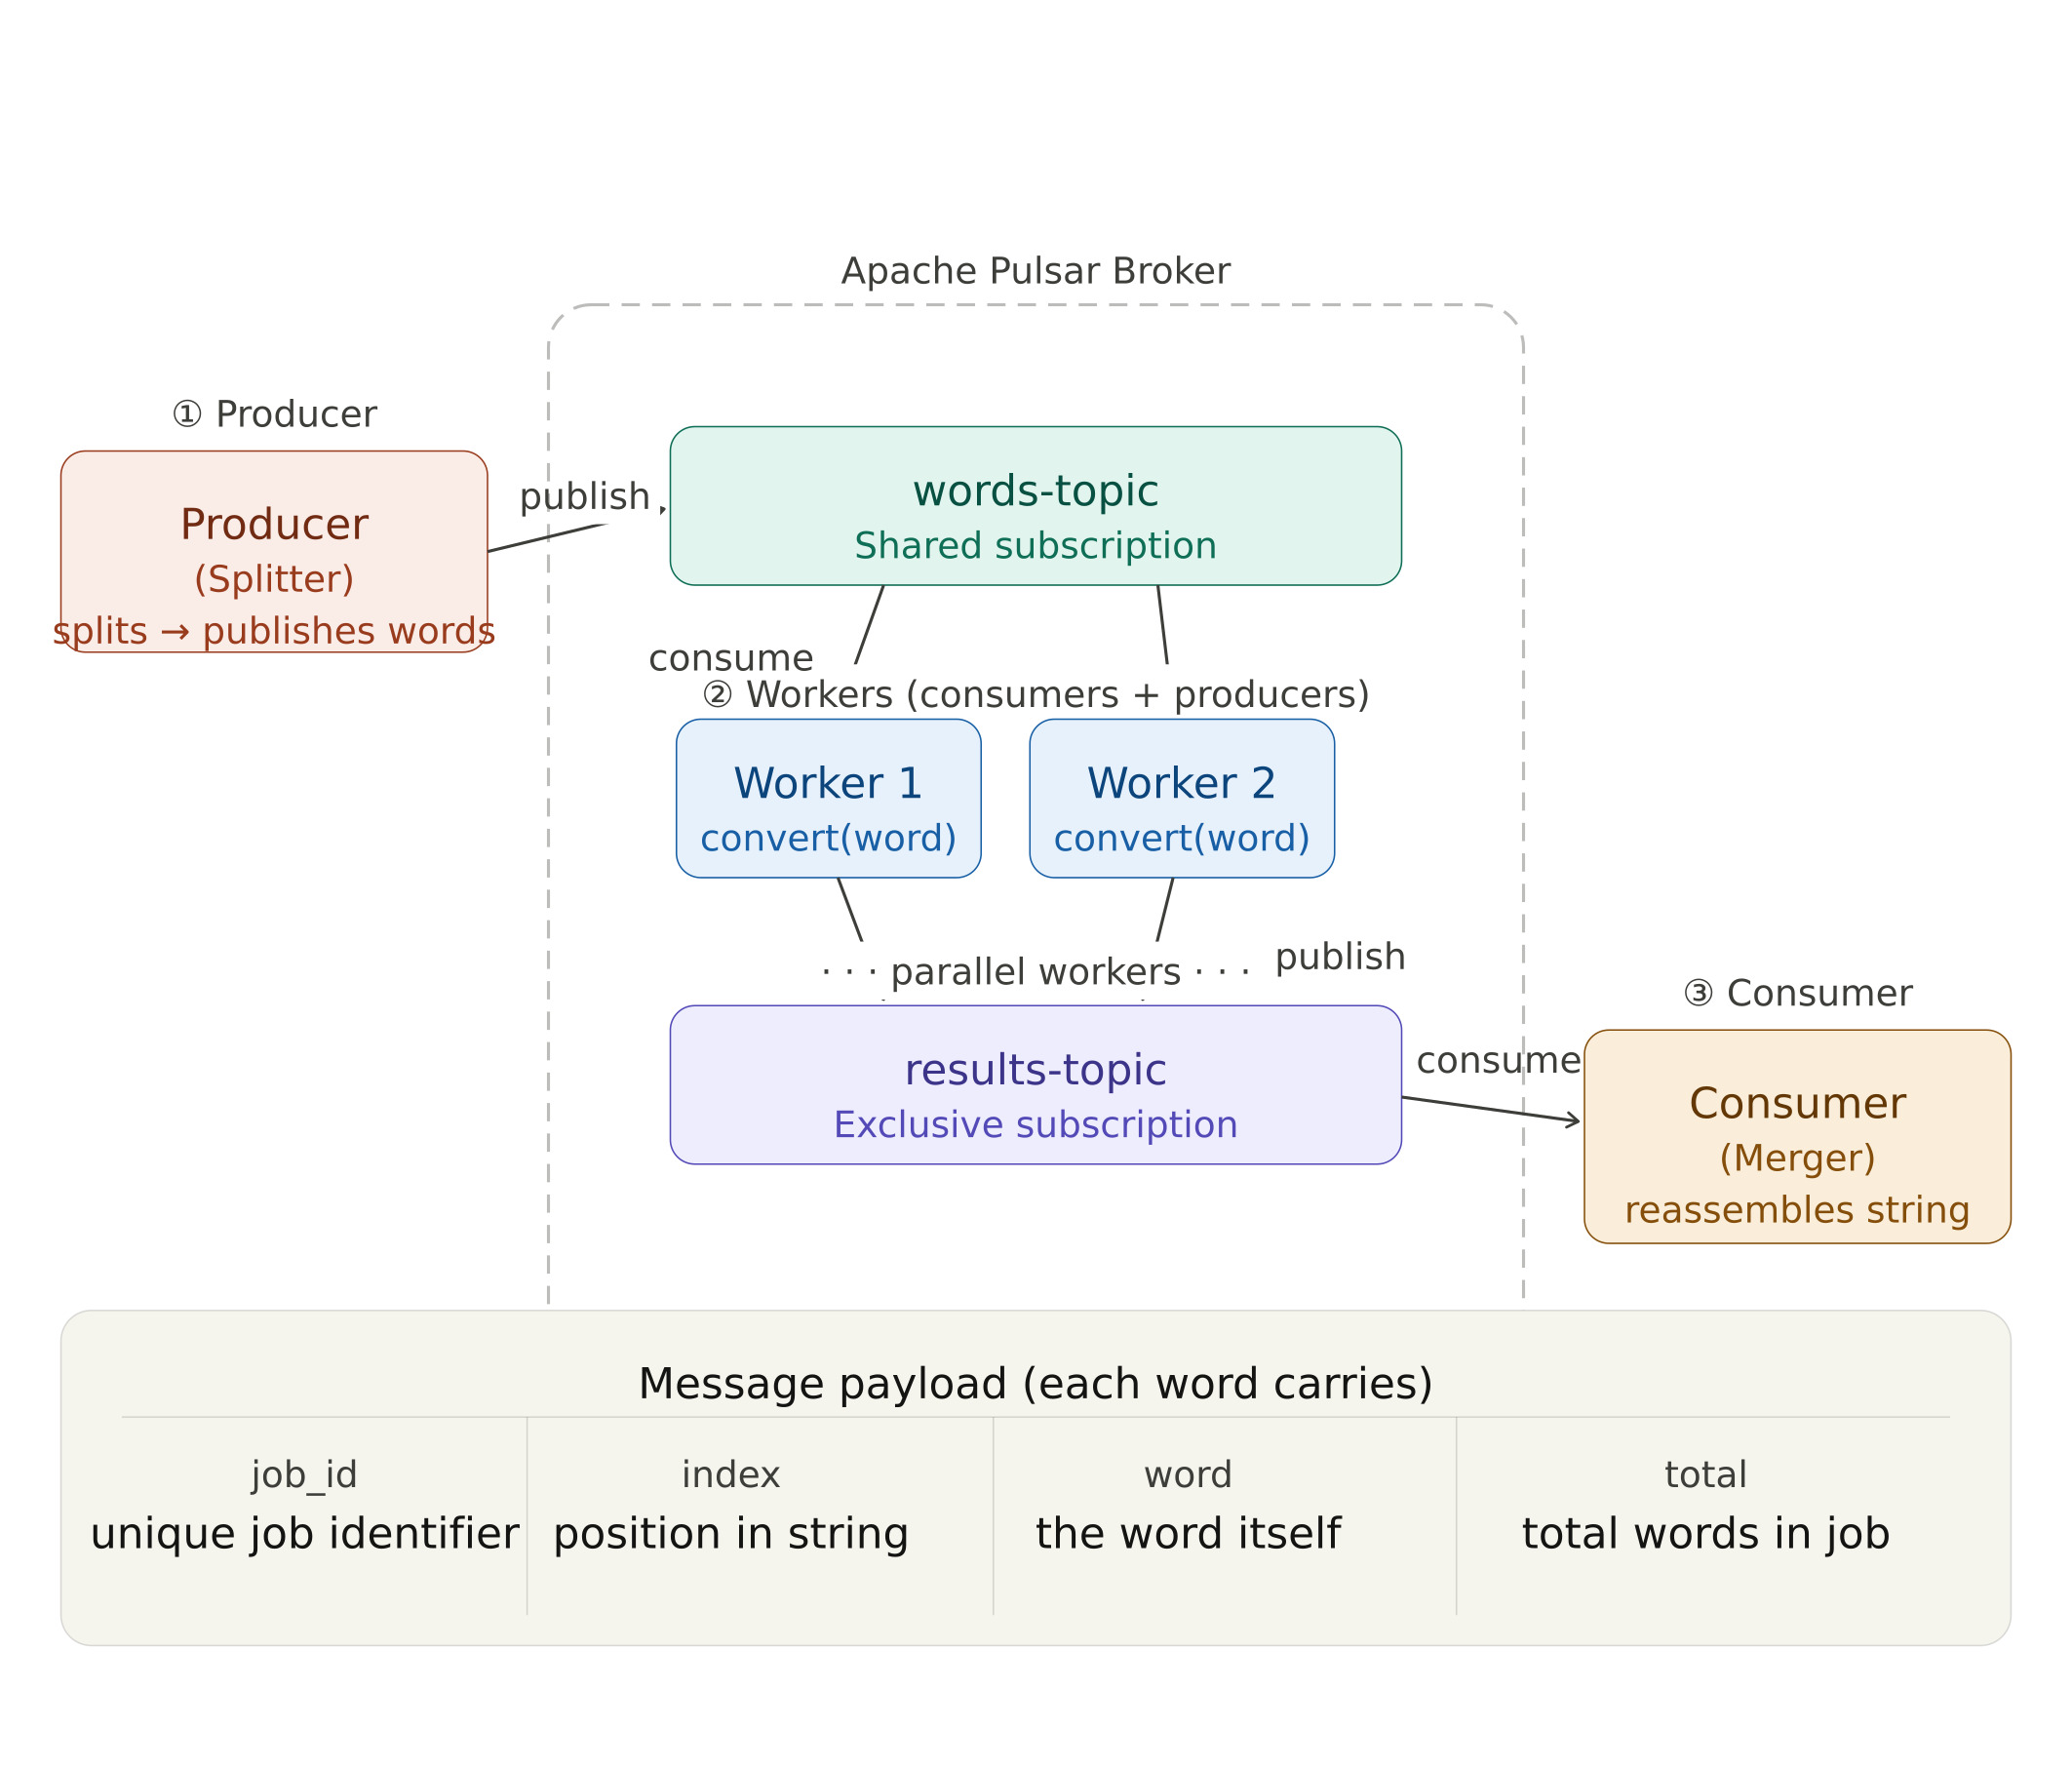
\includegraphics[width=\textwidth]{apache_pulsar_pipeline_architecture.jpg}
  \caption{Architecture of the redesigned Pulsar pipeline: the producer splits the input
  into words, workers process them in parallel via a Shared subscription, and the merger
  reassembles the final output.}
  \label{fig:pipeline-architecture}
\end{figure}

\subsection{Implementation}

The implementation consists of three Python files:

\begin{itemize}[leftmargin=1.5cm]
  \item \texttt{producer-task-4.py}: splits the input string and publishes words to \texttt{words-topic}
  \item \texttt{consumer-task-4-worker.py}: applies conversion function and forwards results to \texttt{results-topic}
  \item \texttt{consumer-task-4-merger.py}: collects results from \texttt{results-topic} and reassembles the final string
\end{itemize}

The implementation details are shown in Appendix \ref{app:code}.

\subsection{Running the Programs}

All three components run on the same VM, each in a separate terminal session (e.g. with
\texttt{tmux}). Pulsar must already be running before starting any of the components.

\begin{lstlisting}[style=shell, caption={Starting the merger, worker, and producer in separate sessions}]
# Session 1: start the merger first so it is ready to collect results
python3 consumer-task-4-merger.py

# Session 2: start worker
python3 consumer-task-4-worker.py

# Session 3: run the producer to split and publish the input string
python3 producer-task-4.py
\end{lstlisting}

The producer splits the input string into words and publishes them to \texttt{words-topic}.
The worker picks up each word, converts it to uppercase, and
publishes the result to \texttt{results-topic}. The merger collects all converted words and,
once it has received all words for the job, prints the final reconstructed string.

\begin{figure}[h!]
  \centering
  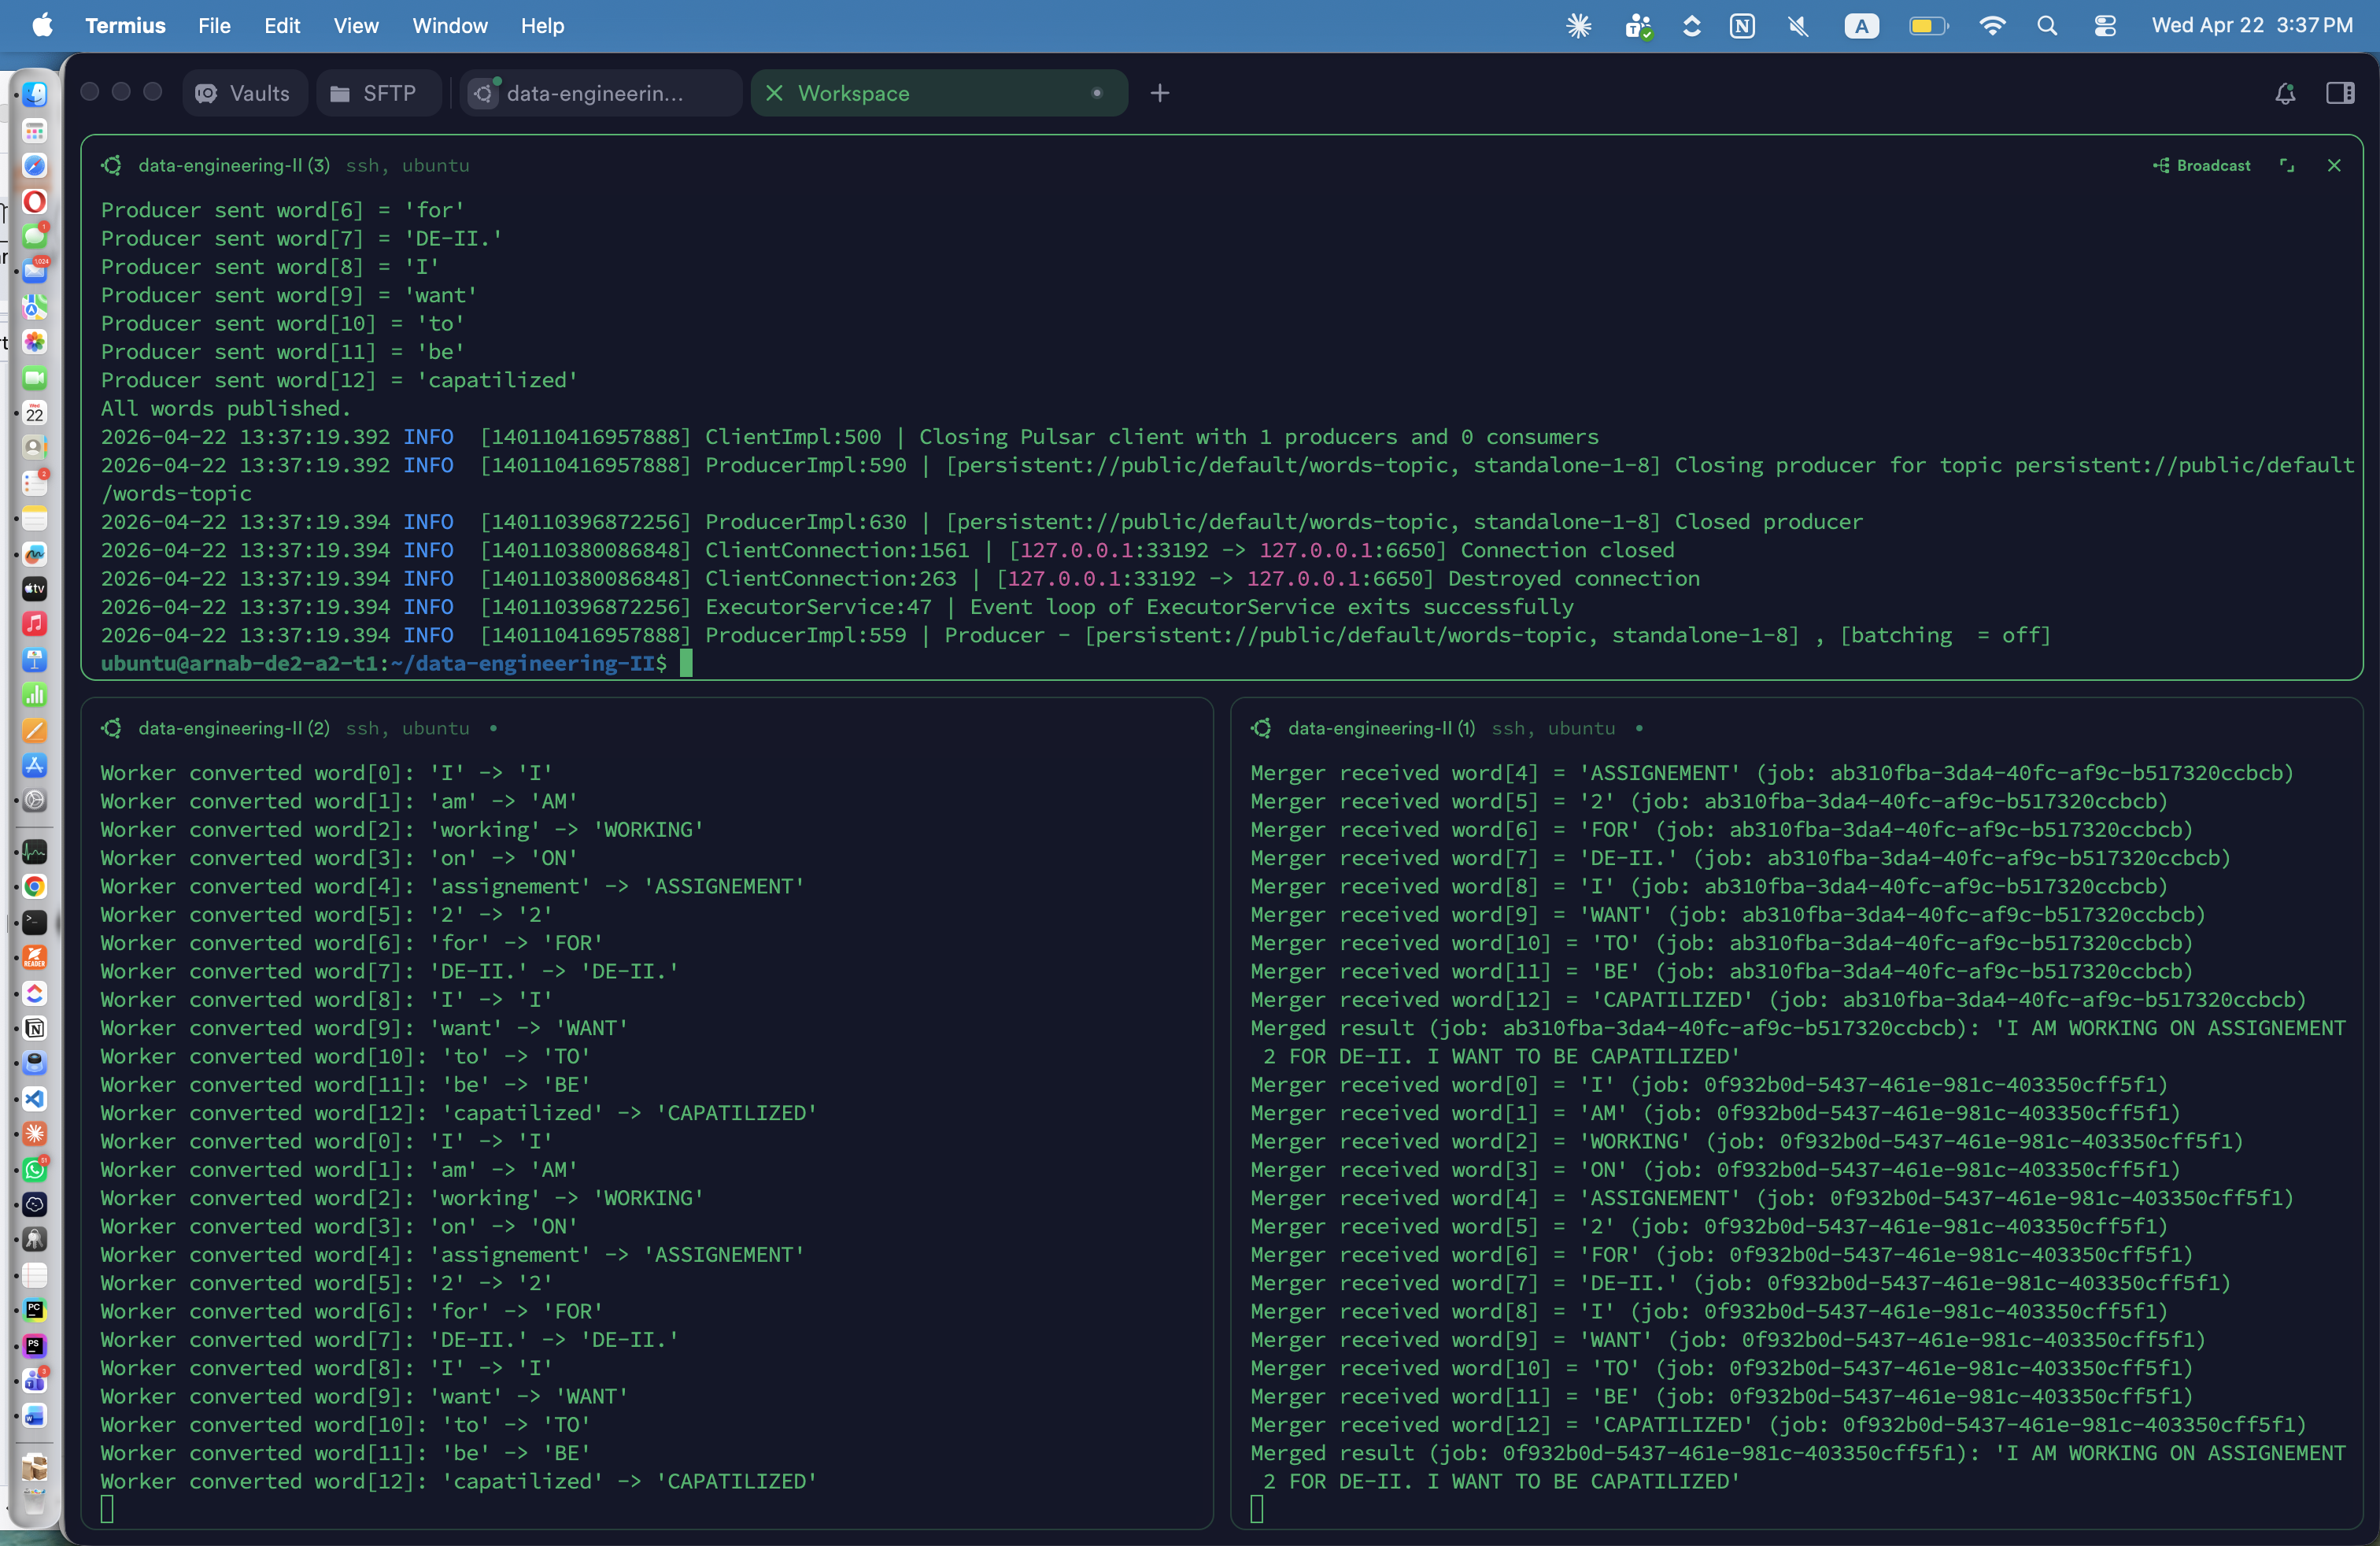
\includegraphics[width=\textwidth]{task-4.png}
  \caption{Task 4 running on a single VM: the producer splits the input string, the worker
  converts each word to uppercase, and the merger reassembles the converted string.}
  \label{fig:task4}
\end{figure}

\newpage
% =============================================================================
\begin{appendices}
\section{Code Files}
\label{app:code}
% =============================================================================

\subsection{Task 2.A: Consumer}

\lstinputlisting[style=python, caption={consumer-task-2-A.py}]{../consumer-task-2-A.py}

\subsection{Task 2.A: Producer}

\lstinputlisting[style=python, caption={producer-task-2.py}]{../producer-task-2.py}

\subsection{Task 2.B: Consumer}

\lstinputlisting[style=python, caption={consumer-task-2-B.py}]{../consumer-task-2-B.py}

\subsection{Task 4: Producer}

\lstinputlisting[style=python, caption={producer-task-4.py}]{../producer-task-4.py}

\subsection{Task 4: Worker}

\lstinputlisting[style=python, caption={consumer-task-4-worker.py}]{../consumer-task-4-worker.py}

\subsection{Task 4: Merger}

\lstinputlisting[style=python, caption={consumer-task-4-merger.py}]{../consumer-task-4-merger.py}

\section{VM Setup Script}
% =============================================================================

I used the following script to provision the VM with all required dependencies
before running Pulsar and the Python programs.

\lstinputlisting[style=shell, caption={setup\_vm.sh}]{../setup_vm.sh}

\end{appendices}
% =============================================================================
\end{document}
